\documentclass[sigconf,nonacm]{acmart}
\settopmatter{printacmref=false,printfolios=true}
\setcopyright{none}
\renewcommand\footnotetextcopyrightpermission[1]{}
\usepackage{amsmath,tabularx,array,enumitem,balance,tikz}
\usetikzlibrary{arrows.meta,positioning,shapes.geometric}
\definecolor{CourseBlue}{HTML}{315EFB}
\definecolor{CourseTeal}{HTML}{14877D}
\definecolor{CourseInk}{HTML}{18324A}
\hypersetup{colorlinks=true,linkcolor=CourseBlue,citecolor=CourseTeal,urlcolor=CourseTeal}
\newcolumntype{Y}{>{\raggedright\arraybackslash}X}
\setlist{leftmargin=*,topsep=3pt,itemsep=2pt}
\newcommand{\CourseNumber}{COMSCI/ECON 206}
\newcommand{\CourseName}{Computational Microeconomics}
\newcommand{\CourseSession}{Autumn 2026 Session 1}
\newcommand{\Instructor}{Professor Luyao Zhang}
\newcommand{\TeamCode}{FP4}
\newcommand{\SymposiumSession}{}
\newcommand{\GitHubLink}{public in the course organization (\texttt{PS2-FP4-CapabilityTransfer}); the submitted artifact is \texttt{code/distill\_sim.py} in this package}
\newcommand{\NotebookLink}{\texttt{python code/distill\_sim.py}, deterministic, seed 206; no hosted notebook yet}
\newcommand{\HuggingFaceLink}{built: the peer-play interface is live as the Space \texttt{FP4\_PS2}, designed in Section~4}
\newcommand{\PosterLink}{exported: \texttt{PS2-FP04-CapabilityTransfer-A0-Poster.pptx / .pdf}; the claim and the subsidy case follow Sections~4--5}
\newcommand{\coursemeta}{\noindent\textbf{Submission to:} \CourseNumber{} --- \CourseName.\\
\textbf{Course session:} \CourseSession. \textbf{Team:} \TeamCode.\\
\textbf{Course instructor:} \Instructor. \textbf{Assignment:} PS2 collaborative research proposal.\par\smallskip}
\title{Pay for Training, Not for Openness: Reward Design for Original and Distilled AI Models}
\author{Zhengjun He}
\affiliation{\institution{Duke Kunshan University}\city{Kunshan}\country{China}}
\email{zhengjun.he@dukekunshan.edu.cn}
\author{Yichen Shen}
\affiliation{\institution{Duke Kunshan University}\city{Kunshan}\country{China}}
\email{yichen.shen@dukekunshan.edu.cn}
% Third author slot left blank: add \author{...}, \affiliation{...}, \email{...} when known.
\renewcommand{\shortauthors}{Team \TeamCode}

% The instructor is course metadata, not a paper author.
% The annotated driver keeps this same paper layout and adds a printable side rail.
\newif\ifTeachingAnnotations
\TeachingAnnotationstrue
% Visible, printable teaching notes. The original ACM text area is unchanged.
% Use main.tex for the clean submission and annotated.tex for guidance.
\ifTeachingAnnotations
\usepackage{eso-pic,tikz}
\usepackage[most]{tcolorbox}
\definecolor{AnnReplace}{HTML}{245BB4}
\definecolor{AnnConnect}{HTML}{08756C}
\definecolor{AnnDevelop}{HTML}{79469C}
\definecolor{AnnInk}{HTML}{21324A}
\definecolor{AnnRail}{HTML}{F4F6FA}
\definecolor{AnnLine}{HTML}{D4DCE7}
\newsavebox{\AnnRailBox}
\newcommand{\AnnNote}[4]{%
  \begin{tcolorbox}[enhanced,sharp corners,boxrule=0pt,frame hidden,
    colback=#2!5!white,borderline west={2pt}{0pt}{#2},
    left=7pt,right=7pt,top=5pt,bottom=5pt,before skip=6pt,after skip=0pt]
    \sffamily\fontsize{9.4}{11.8}\selectfont\color{AnnInk}\raggedright
    {\color{#2}\bfseries #1\quad #3}\par\vspace{2pt}#4
  \end{tcolorbox}}
\newcommand{\AnnPin}[4]{%
  \node[rounded corners=2bp,fill=#2,text=white,inner xsep=4bp,
    inner ysep=2.5bp,font=\sffamily\bfseries\fontsize{8}{9}\selectfont]
    at (#3,#4) {#1};}
\newcommand{\AnnPageTitle}{%
  \ifcase\value{page}\or
    Keep the PS1 structure\or
    Integrate evidence and impact\or
    Preserve the appendix sequence\or
    Update the same cumulative map\or
    Add only the PS2 extension record\else
    Continue the documented draft\fi}
\newcommand{\AnnPageNotes}{%
  \ifcase\value{page}\or\AnnNote{R1}{AnnReplace}{Replace team identity, not course identity}{%
Replace the title, team code, symposium session, member names, and emails. Keep the course, term, and \textbf{Course instructor: Professor Luyao Zhang}. The instructor is metadata, not a paper author.}

\AnnNote{R2}{AnnReplace}{Adapt the LaTeX-native teaser}{%
Edit \texttt{figures/ps2\_teaser.tex}. Keep the three evidence panels and synthesis logic, but replace their content with your actors, model, computation, behavioral test, A0-poster claim, and real-world case.}

\AnnNote{C1}{AnnConnect}{Keep the familiar five-section spine}{%
Section 1 asks the connected questions. Sections 2--4 answer the economics, computation, and behavior questions. Section 5 states the integrated contribution and practical impact. Carry the same claims into Appendix E.}

\AnnNote{D1}{AnnDevelop}{Choose the correct solution concept}{%
Define players, strategies, timing, information, beliefs, and payoffs before naming an equilibrium. Translate the same problem through game theory, social choice, and mechanism design; show what changes.}
\or
    \AnnNote{C2}{AnnConnect}{Make behavioral evidence consequential}{%
Use self-reflection and peer play to probe an assumption. State the competing explanation and the observation that would make the team retain, qualify, or revise the model, algorithm, or interface.}

\AnnNote{D2}{AnnDevelop}{Connect the real-world case to evidence}{%
Identify stakeholders, feasible benefit, risk, missing evidence, and correction route. Compare the standards of academia, industry, and public institutions without claiming impact that has not been measured.}

\AnnNote{R3}{AnnReplace}{Use the confirmed dates}{%
Review-ready: September 27 at 11:00 P.M. Symposium, peer evaluation, and practical-impact discussion: September 28. Final revision: September 30 at 11:00 P.M., before the October 1--2 holiday.}
\or\AnnNote{R4}{AnnReplace}{Credit people and work accurately}{%
Keep Professor Luyao Zhang as course instructor. Acknowledge peers, discussants, partners, data, software, adapted materials, and AI assistance only when used. Give each author an inspectable intellectual decision and output.}

\AnnNote{D3}{AnnDevelop}{Appendices A and B remain familiar}{%
Appendix A holds technical details, reproducibility, and AI disclosure. Appendix B retains the PS1 change record: earlier claim, dated evidence or feedback, revision, and intellectual consequence.}

\AnnNote{C3}{AnnConnect}{Appendices C and D preserve continuity}{%
Appendix C records open-source inspirations and the three-lens stress test. Appendix D preserves review, response, rerun, and revision. Do not replace missing feedback with invented evidence.}
\or
    \AnnNote{R5}{AnnReplace}{Complete the same eight rows}{%
Appendix E deliberately retains the PS1 structured abstract. Replace each prompt, save the prior version, and use complete, specific sentences.}

\AnnNote{C4}{AnnConnect}{Rows 1--4 must match Sections 1--3}{%
Use the same gap, application, connected questions, actors, incentives, timing, information, baseline, and evidence status. A reader should not encounter a different model in the table.}

\AnnNote{D4}{AnnDevelop}{Rows 5--8 close the evidence loop}{%
Separate actual and expected results. Explain the integrated intellectual merit and bounded practical impact. Record the dated feedback, revision location, verification, and consequence.}
\or\AnnNote{D5}{AnnDevelop}{Record the auction, not only the outcome}{%
State values or signals, prediction, bid, allocation, payment, stopping rule, utility, revenue, efficiency, behavioral observation, and revision for each treatment.}

\AnnNote{C5}{AnnConnect}{Check parity across three artifacts}{%
GitHub, Hugging Face, and the A0 poster must describe the same question, model, evidence status, result, and limits. The labels describe evidence perspectives, not fixed team roles.}

\AnnNote{D6}{AnnDevelop}{Use the symposium to revise}{%
Retain the September 28 poster and reviews. Record Keep, Revise, or Investigate decisions, rerun the affected check, and identify the exact September 30 change.}
\else
    \AnnNote{D}{AnnDevelop}{Return to the clean driver}{Use \texttt{main.tex} for submission. Recheck the two-page main limit and preserve supporting evidence in the appendices.}
  \fi}
\newcommand{\AnnPagePins}{%
  \ifcase\value{page}\or
    \AnnPin{R1}{AnnReplace}{31}{88}
    \AnnPin{R2}{AnnReplace}{31}{370}
    \AnnPin{C1}{AnnConnect}{31}{510}
    \AnnPin{D1}{AnnDevelop}{581}{400}
  \or
    \AnnPin{C2}{AnnConnect}{31}{94}
    \AnnPin{D2}{AnnDevelop}{31}{240}
    \AnnPin{R3}{AnnReplace}{581}{340}
  \or
    \AnnPin{R4}{AnnReplace}{31}{105}
    \AnnPin{D3}{AnnDevelop}{31}{390}
    \AnnPin{C3}{AnnConnect}{581}{240}
  \or
    \AnnPin{R5}{AnnReplace}{31}{92}
    \AnnPin{C4}{AnnConnect}{31}{260}
    \AnnPin{D4}{AnnDevelop}{31}{420}
  \or
    \AnnPin{D5}{AnnDevelop}{31}{92}
    \AnnPin{C5}{AnnConnect}{31}{310}
    \AnnPin{D6}{AnnDevelop}{581}{260}
  \fi}
\AddToHook{shipout/before}{\global\pdfpagewidth=912bp\relax}
\AddToShipoutPictureBG{\AtPageUpperLeft{%
  \begin{tikzpicture}[overlay,x=1bp,y=-1bp]
    \fill[AnnRail] (612,0) rectangle (912,792);
    \draw[AnnLine,line width=.6bp] (612,0)--(612,792);
  \end{tikzpicture}}}
\AddToShipoutPictureFG{\AtPageUpperLeft{%
  \savebox{\AnnRailBox}{\normalfont\begin{minipage}[t]{266bp}\AnnPageNotes\end{minipage}}
  \begin{tikzpicture}[overlay,x=1bp,y=-1bp]
    \AnnPagePins
    \node[anchor=north west,inner sep=0,text width=266bp] at (629,26) {%
      \sffamily\color{AnnInk}\fontsize{10}{12}\selectfont\raggedright
      \textbf{PS2 / ANNOTATED WORKING COPY}\par\vspace{5pt}
      {\fontsize{15}{17}\selectfont\bfseries\AnnPageTitle}\par\vspace{7pt}
      {\fontsize{9}{11}\selectfont
      \textcolor{AnnReplace}{\textbf{R REPLACE}}\quad
      \textcolor{AnnConnect}{\textbf{C CONNECT}}\quad
      \textcolor{AnnDevelop}{\textbf{D DEVELOP}}}};
    \node[anchor=north west,inner sep=0] at (629,102) {\usebox{\AnnRailBox}};
    \node[anchor=north west,inner sep=0,text width=266bp] at (629,748) {%
      \sffamily\fontsize{8.4}{10.2}\selectfont\color{AnnInk}
      Guidance is scaffolding. Submit from \texttt{main.tex}.
      \textbf{\thepage/5}};
  \end{tikzpicture}}}
\fi


\begin{document}
\begin{teaserfigure}
\captionsetup{skip=8pt}
\centering
\resizebox{0.70\textwidth}{!}{%
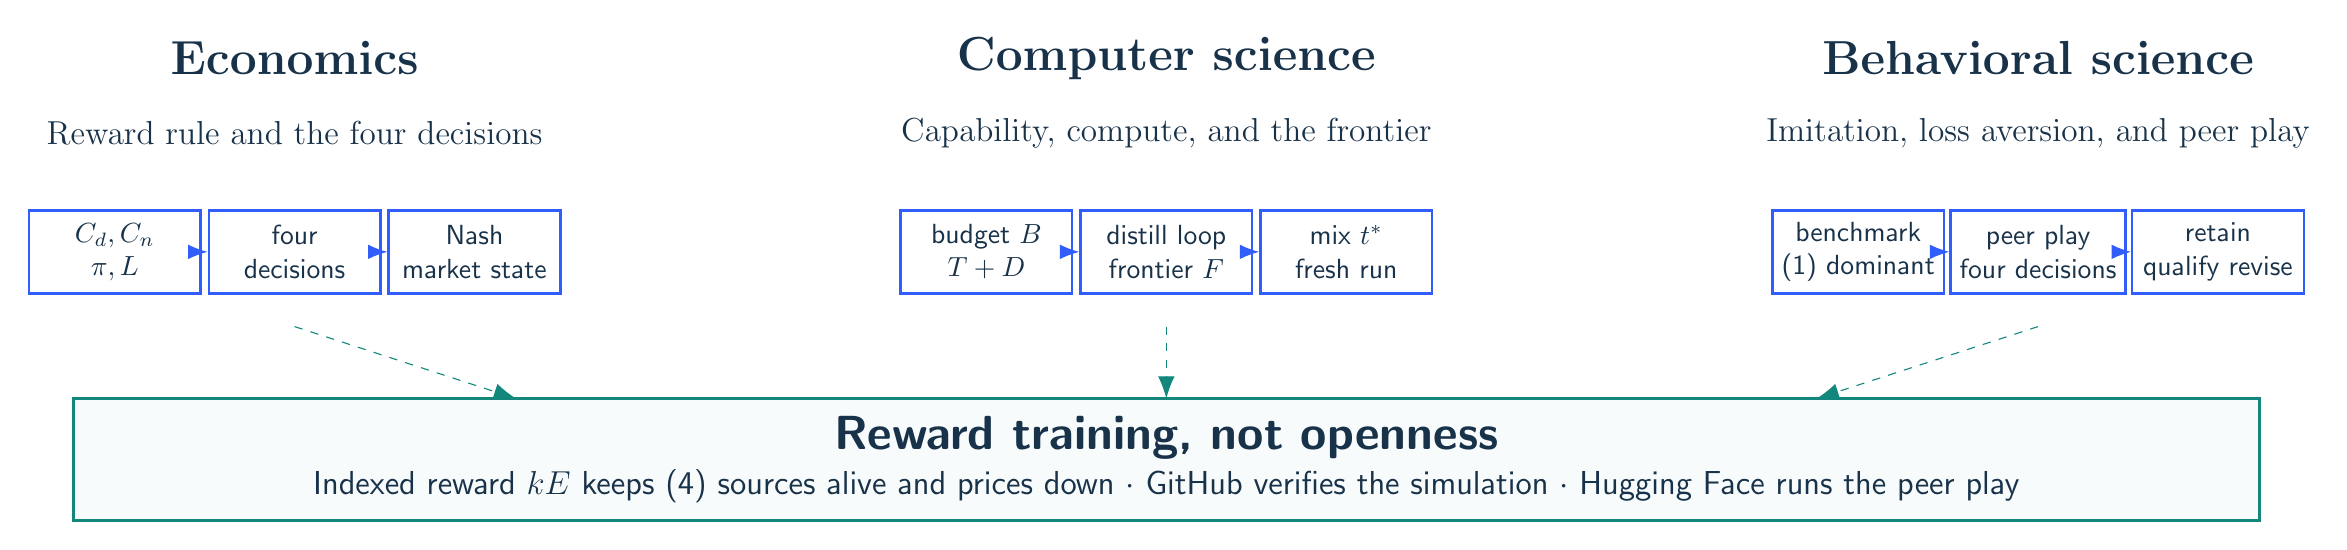
\begin{tikzpicture}[x=1pt,y=1pt,font=\sffamily,>=Latex]
\tikzset{
  heading/.style={font=\bfseries\fontsize{18}{20}\selectfont,text=CourseInk,align=center},
  label/.style={font=\fontsize{12}{14}\selectfont,text=CourseInk,align=center},
  mini/.style={draw=CourseBlue,line width=0.9pt,minimum width=62pt,minimum height=30pt,align=center,text=CourseInk,fill=white},
  synthesis/.style={draw=CourseTeal,line width=1.1pt,minimum width=790pt,minimum height=44pt,align=center,text=CourseInk,fill=CourseTeal!3}
}
\node[heading] at (140,190) {Economics};
\node[label] at (140,163) {Reward rule and the four decisions};
\node[mini] (e1) at (75,120) {$C_d,C_n$\\$\pi,L$};
\node[mini] (e2) at (140,120) {four\\decisions};
\node[mini] (e3) at (205,120) {Nash\\market state};
\draw[CourseBlue,-{Latex[length=7pt]}] (e1)--(e2);
\draw[CourseBlue,-{Latex[length=7pt]}] (e2)--(e3);

\node[heading] at (455,190) {Computer science};
\node[label] at (455,163) {Capability, compute, and the frontier};
\node[mini] (c1) at (390,120) {budget $B$\\$T+D$};
\node[mini] (c2) at (455,120) {distill loop\\frontier $F$};
\node[mini] (c3) at (520,120) {mix $t^\ast$\\fresh run};
\draw[CourseBlue,-{Latex[length=7pt]}] (c1)--(c2);
\draw[CourseBlue,-{Latex[length=7pt]}] (c2)--(c3);

\node[heading] at (770,190) {Behavioral science};
\node[label] at (770,163) {Imitation, loss aversion, and peer play};
\node[mini] (b1) at (705,120) {benchmark\\(1) dominant};
\node[mini] (b2) at (770,120) {peer play\\four decisions};
\node[mini] (b3) at (835,120) {retain\\qualify revise};
\draw[CourseBlue,-{Latex[length=7pt]}] (b1)--(b2);
\draw[CourseBlue,-{Latex[length=7pt]}] (b2)--(b3);

\node[synthesis] (s) at (455,45) {\textbf{\fontsize{17}{19}\selectfont Reward training, not openness}\\[3pt]
\fontsize{12}{14}\selectfont Indexed reward $kE$ keeps (4) sources alive and prices down $\cdot$ GitHub verifies the simulation $\cdot$ Hugging Face runs the peer play};
\draw[CourseTeal,dashed,-{Latex[length=8pt]}] (140,93)--(220,67);
\draw[CourseTeal,dashed,-{Latex[length=8pt]}] (455,93)--(455,67);
\draw[CourseTeal,dashed,-{Latex[length=8pt]}] (770,93)--(690,67);
\end{tikzpicture}}

\caption{One integrated PS2 evidence chain. Economic reasoning defines the strategic question and institutional objective; reproducible computation tests the model; behavioral evidence probes assumptions; the A0 poster communicates the combined claim and its practical implications for a concrete real-world case. Replace every placeholder and distinguish completed evidence from planned work.}
\Description{Three disciplinary panels for economics, computer science, and behavioral science flow into an interdisciplinary synthesis bar linking the strategic claim, GitHub evidence, Hugging Face evidence, A0 poster, and real-world impact.}
\label{fig:teaser}
\end{teaserfigure}
\maketitle\raggedbottom\coursemeta

\noindent\textcolor{CourseTeal}{\textbf{Annotated working copy.}} This driver keeps the submission layout and adds a printable guidance rail. Submit from \texttt{main.tex}. Keep Sections 1--5 within two main pages, including metadata, Figure~\ref{fig:teaser}, its caption, and the artifact links.

\section{Three connected research questions and verified gap}
A firm builds a model by training from scratch at cost $C_n$, or by distilling an existing model at cost $C_d\ll C_n$~\cite{hinton2015,acl2024distill}. It keeps the model closed for monopoly profit $\pi$, or releases it openly for a reward $kE$ --- coefficient $k$ times the training compute $E$ of the release --- while losing exclusivity at cost $L$.

Today's rules reward \emph{openness}, so a distilled copy and an original source earn the same~\cite{qiu2025,epoch2025}. The market then settles in state 1 (all closed), state 2 (all distilled: no source, no new capability), or state 3 (healthy: enough sources, reasonable price). Verified gap: the nearest studies compare open with closed models~\cite{epoch2025} or model open sourcing~\cite{habibi2025}, but none compares a lump-sum openness reward with a compute-indexed reward over the same four decisions.

\textbf{Q1---Economics:} Which reward rule aligns the private and social rankings of the four decisions?\par
\textbf{Q2---Computation:} Does distillation create capability, or only spend compute?\par
\textbf{Q3---Behavior:} What does each decision pay a firm, and how does it learn which one to choose?\par
Shared question: can an $E$-indexed reward hold state 3, at what $k$, and what share of compute should go to training? Figure~\ref{fig:teaser} links the three answers.

\section{Answer to Q1: incentives and strategic model}
Players: $N$ firms; actions $\{$closed, open$\}\times\{$distill, train$\}$; one simultaneous move; common-knowledge parameters, with the cost multiplier and market power drawn before play and not hidden strategically; objective: own payoff; solution concept: dominant strategies, then Nash equilibrium~\cite{nash1950,selten1975,harsanyi1968,osborne1994,fudenberg1991}. Table~\ref{tab:four} gives the four decisions.

\begin{table}[h]\caption{The four decisions, their payoffs, and the reversed rankings (1 = most wanted). An open release also keeps the future market share it buys, $\beta\phi K\,m/(m{+}m_0)$ --- the Future column, the discounted value of the external contributions an open model attracts~\cite{habibi2025,xu2025}.}
\label{tab:four}
\footnotesize\setlength{\tabcolsep}{3.5pt}\renewcommand{\arraystretch}{1.02}
\begin{tabularx}{\columnwidth}{@{}p{1.85cm}p{2.05cm}p{0.95cm}ccY@{}}\toprule
\textbf{Decision}&\textbf{Payoff}&\textbf{Future}&\textbf{Priv.}&\textbf{Soc.}&\textbf{Reading}\\\midrule
(1) closed, distill&$-C_d+\pi$&$0$&1&4&free rider~\cite{olson1965}\\
(2) open, distill&$-C_d+kE_d-L$&$\beta\phi K$&3&2&passer-on\\
(3) closed, train&$-C_n+\pi$&$0$&2&3&monopolist\\
(4) open, train&$-C_n+kE_n-L$&$\beta\phi K$&4&1&source\\\bottomrule
\end{tabularx}\end{table}

At $\beta\phi K=0$ the private ranking $(1)\succ(3)\succ(2)\succ(4)$ exactly reverses the social ranking $(4)\succ(2)\succ(3)\succ(1)$: the privately best decision is cheap and exclusive but destroys the source: knowledge is non-rival, so private returns fall short of social returns~\cite{arrow1962,romer1990}. Without policy the market stops at (1), a dominant strategy at $k=0$.

Tool 1 rewards openness only, so (2) beats (4) at every $R$: nobody trains, sources run out, state 2. Tool 2 indexes the reward by training compute, $kE$: (4) has large $E$, (2) has small $E$, and (1) and (3) receive nothing. Table~\ref{tab:design} reports the fresh run.

The future-share motive changes where an unregulated market settles. With it on, firms release weights with no reward at all, because openness buys a place in the next generation of infrastructure: at $k=0$ the share of firms opening rises from $0.00$ to $0.68$ and the market settles in state 2 rather than state 1 --- firms open, but what they open is a copy. Opening pays exactly for firms whose share of compatible applications lies between the two roots of $\beta\phi K\,m/(m+m_0)=L+\pi m$, the inverted-U relation the literature reports~\cite{habibi2025,xu2025}. The indexed reward still reaches state 3, and the cap still returns the market to state 2. \begin{table}[h]\caption{Reward design and market outcome (fresh run, $N=20000$, seed 206), share of firms per decision.}
\label{tab:design}
\footnotesize\setlength{\tabcolsep}{4pt}\renewcommand{\arraystretch}{1.02}
\begin{tabularx}{\columnwidth}{@{}p{1.85cm}Yp{1.35cm}@{}}\toprule
\textbf{Reward rule}&\textbf{(1)/(2)/(3)/(4)}&\textbf{State}\\\midrule
\multicolumn{3}{@{}l}{\emph{(a) no future-share motive, $\beta\phi K=0$}}\\
none, $k=0$&.96 / .00 / .04 / .00&1 closed\\
openness, $R=20$&.11 / .85 / .00 / .04&2 distill\\
indexed, $k=4$&.35 / .00 / .01 / .64&3 healthy\\
indexed, capped, $k=12$&.42 / .54 / .02 / .03&2 distill\\\midrule
\multicolumn{3}{@{}l}{\emph{(b) with the future-share motive, $\beta\phi K=19.98$}}\\
none, $k=0$&.28 / .68 / .01 / .03&2 distill\\
openness, $R=20$&.01 / .95 / .00 / .04&2 distill\\
indexed, $k=4$&.03 / .02 / .00 / .95&3 healthy\\
indexed, capped, $k=12$&.03 / .93 / .00 / .05&2 distill\\\bottomrule
\end{tabularx}\end{table}

The thresholds are analytic. Disclosure needs $kE_d+\beta\phi K\,m/(m+m_0)>L+\pi m$: with the motive off this is $k>(L+\pi)/E_d$ (the familiar $k>L$ assumed $\pi=0$), and with a strong motive disclosure pays at $k=0$. Innovation needs $k>\Delta C/\Delta E$, the cost and compute gaps between training and distilling, and this threshold is unaffected by the future-share motive because the term is common to both open cells~\cite{wright1983,nalebuff1983}. Appendix~C carries the three lenses.

\section{Answer to Q2: computation, auction comparison, and artifacts}
Openness is not only what a weight release produces. A model served through an interface is distilled by whoever queries it, at industrial scale~\cite{cisa2026}, so distillation is itself a degree of openness --- and a firm that bans accounts, caps usage, or writes distillation out of its terms is buying exclusivity back. Countermeasures are the mirror image of openness: the harder they bind, the less open the model really is, and a firm can move that quantity without releasing or withholding a single weight. We keep the release move binary --- the closed cell is the case where countermeasures fully bind and their cost sits inside $L$ --- but the reward is an all-pay auction~\cite{baye1996}: each firm's bid is its audited training compute $E$, every firm pays it because training is sunk whether or not it wins, and the prize goes to the highest verified $E$. Our rule pays proportionally instead ($kE$ per open release), so the analogy covers the payment side, not the allocation form. All-pay auctions dissipate rents, which is why the cap matters~\cite{baye1999,tullock1980}; the bid is real compute, verifiable only by audit~\cite{sastry2024}.

Model: budget $B=T+D$ for training $T$ and distillation $D$; only training moves the frontier $F(T)=1-e^{-T/T_0}$~\cite{kaplan2020,hoffmann2022}, while distillation copies it with loss $\delta<1$. Metrics: decision shares, market state, and social loss $c_eB+\rho\max(0,T-T_0)-vF(T)$, with $\rho$ pricing duplicated effort~\cite{dasgupta1980} and $v$ the frontier. Pseudocode: draw each firm's type, evaluate the four payoffs, take the logit best response~\cite{mckelvey1995}, aggregate to the market state; seed 206, with parameters and output in Appendix~A.

Fresh run (Appendix~A). Mutual distillation burns $500$ compute units while the frontier falls from $1.000$ to $0.774$: copying a copy only decays~\cite{shumailov2024}. In the budget account, social loss is lowest at a training share of $t^\ast=0.35$ ($+1.35$), against $+2.00$ for all distill and $+1.77$ for all train, so a positive distillation share is efficient. Planned: estimate $T_0$, $\rho$, $\delta$.

\textbf{GitHub:} \GitHubLink\\
\textbf{Notebook:} \NotebookLink\\
\textbf{Hugging Face:} \HuggingFaceLink\\
\textbf{A0 poster:} \PosterLink

\section{Answer to Q3: behavior and interdisciplinary integration}
Rational benchmark: payoff maximization, with (1) dominant at $k=0$. 
Table~\ref{tab:four} gives what each decision pays the firm and does to the market.

Behavioral mechanism: firms imitate the cheapest visible profitable action, so imitation pushes the market from (1) toward (2); loss aversion makes the lost exclusivity $L$ weigh more than an equal reward $kE$~\cite{kahneman1979}, so firms under-open. Competing explanation: firms release open weights for reputation and future market share, so openness is cheaper than a model without the $\beta\phi K$ term assumes~\cite{lerner2002,vonhippel2003,fosfuri2008,habibi2025}. Distinguishing observation: hold total reward spending fixed and switch from lump sum to $E$-indexed --- if imitation dominates, the share of (4) rises slowly; under reputation, the switch changes little. The Hugging Face game runs this switch as peer play; if imitation dominates, we retain the model but qualify common knowledge.

\section{Advanced development, real-world impact, and roadmap}
Foundations: equilibrium reasoning~\cite{nash1950,selten1975,harsanyi1968} (Nobel 1994), mechanism design~\cite{vickrey1961,mirrlees1971,myerson1981,maskin1999} (Nobel 1996, 2007), and knowledge distillation~\cite{hinton2015} (Turing Award 2018). Distinctive now: weights are copied at almost no cost while training stays expensive.

Real-world case: an agency paying for open-weight models, such as a national compute subsidy. Stakeholders: labs, small firms, users, taxpayers, the agency. Benefits: more sources, lower prices, wider access. Risks: paying for copies, crowding out training, gaming the reward. What counts is audited training compute, not self-declared openness~\cite{sastry2024}; value is original-source releases per unit of spending; the next discriminating test is the reward switch with real firms; the cumulative map is Appendix~E.

\noindent\textbf{Expected 2056 Nobel Prize and Turing Award contribution statement.}
By 2056, we aspire to a reward standard for how society pays for machine intelligence, shown by shifts in original-source releases.

\subsection*{Open Science Statement}
GitHub: \path{code/distill_sim.py}, seed 206, log in \path{code/fresh_run_output.txt}; Hugging Face: Prize Rate Game. Same payoffs and states as this paper.

\subsection*{Statement of Contribution to the UN's SDGs}
Intended contribution to SDG 9.5 and SDG 10: a rule that keeps sources alive widens access, measured by original-source releases per unit of spending~\cite{un_sdg}. Paying for copies would raise spending without new capability.

\subsection*{Submission milestones}
Review-ready September 27, 2026; symposium September 28, 2:45--5:15 P.M., IB 2050; final revision October 6, 2026.

\clearpage\nobalance
\section*{Author Notes}
\subsection*{Acknowledgements}
\textbf{Course instructor: Professor Luyao Zhang.} We thank Professor Zhang for incubating this research from its earliest strategic question, mentoring the interdisciplinary development of the project, and providing formal feedback on PS1. We are grateful to Han Zhang, a Ph.D.\ candidate at Duke University and founder of Liberata, for his feedback on the future market-share incentive incorporated into the revised model. We also thank Mustafa Ayub Khan, Jiayang Sun, and Temur Akhtamjonov for their thoughtful peer reviews at the symposium, and our COMSCI/ECON 206 classmates for collaborative learning and questions. We acknowledge the course Overleaf template, Python, and NumPy. No external model or compute data was used; every number in this paper comes from \path{code/distill_sim.py}. The authors remain responsible for the proposal and any remaining errors.

\subsection*{Team and individual contributions}
\textbf{Joint contribution.} The team asked one question: does rewarding openness buy capability, or only copies? Together we built the four-decision model, defined the two reward tools, and fixed the three market states. We specified a compute account in which only original training moves the capability frontier, and designed the peer-play switch between a lump-sum and an $E$-indexed reward. The simulation, the state classification, the poster claim, and Appendix~D use the same payoffs, parameters, and seed, so every number can be rerun from \path{code/distill_sim.py} at seed 206.

\noindent\textbf{Zhengjun He}, author order 1. \emph{Intellectual decision:} to price training compute rather than openness, and to build the market-competition model that puts both reward rules over the same four decisions. \emph{Output:} \path{code/distill_sim.py} with its saved run, and the market-competition framework of Sections 2--3. \emph{Verification:} reran the simulation at seed 206 and checked that both panels, the compute account and the auction account reproduce; \path{verify_k.py} recomputes the four cells from scratch. \emph{Connection:} the numbers in Table 2, Appendix E and the auction record all come from this model. \emph{Next:} repeated rounds with a declining distillable surplus.

\noindent\textbf{Yichen Shen}, author order 2. \emph{Intellectual decision:} to split the project into the three connected questions --- incentives, computation, behavior --- and to test the behavioral branch as peer play. \emph{Output:} Sections 1 and 4 and the Hugging Face Space, \HuggingFaceLink. \emph{Verification:} ran the Space's reward switch against the paper's payoffs and states and confirmed that each choice maps to its payoff. \emph{Connection:} that switch is the distinguishing observation of Section 4 --- if imitation dominates, the model is kept and common knowledge is qualified. \emph{Next:} log real play in the Space and add repeated rounds.

\bibliographystyle{ACM-Reference-Format}\bibliography{references}
\appendix
\section{Technical details and reproducibility}
Four payoffs per firm, each open cell adding the future term $F(m)=\beta\phi K\,m/(m+m_0)$: (1) $-C_d+\pi$, (2) $-C_d+kE_d-L+F(m)$, (3) $-C_n+\pi$, (4) $-C_n+kE_n-L+F(m)$. Firm types: a simulated population of $N=20000$ firms (no firm-level data enters; the population only aggregates individual choices), cost multiplier $a$ and market power $m$ drawn independently lognormal with $\sigma_a=\sigma_m=0.6$, seed 206, NumPy 2.4.6. Choices use a logit best response with $\lambda=1$~\cite{mckelvey1995}. Level constants, calibrated so that the run reproduces column (a) of Table~\ref{tab:design} (residual $7.4\times10^{-5}$): $C_d=1.4446$, $C_n=5.6704$, $\pi=8.2391$, $L=2.5193$, $E_d=0.9854$, $E_n=4.6311$. Future-share motive: $\beta=0.90$, $\phi=0.50$, $K=44.4$, $m_0=0.50$, giving $\beta\phi K=19.98$~\cite{habibi2025}. Reward designs: (A) lump sum $R$ for any open release; (B) reward $kE$; (C) reward $\min(kE,12)$. Compute account: $F(T)=1-e^{-T/T_0}$, mutual-distillation loop with $\delta=0.95$, $c_d=1$, 100 firms, 5 rounds, and social loss $c_eB+\rho\max(0,T-T_0)-vF(T)$ with $B=100$, $T_0=25$, $\rho=0.01$, $v=1$, $c_e=0.02$. Outputs: \path{code/fresh_run_output.txt}. Shortest reproducible run: \texttt{python code/distill\_sim.py} (in this package). The repository holds \path{k_formula.ipynb}, which derives the two thresholds on $k$ with sympy, and \path{verify_k.py}, which recomputes the four cells from scratch and finds where the best cell changes. Results are deterministic. Known limits: the frontier, duplication price, and $\delta$ are illustrative, not estimated; firms are symmetric except for $a$ and $m$; no entry or exit; no data on real training compute. Repository status: \GitHubLink, release commit \ReleaseCommit.

\subsection{AI-use disclosure}
Generative AI (DeepSeek) was used only for typesetting, for debugging \texttt{distill\_sim.py}, and for locating references. The ideas, the model, and every test and number come from the authors, who reran the code at seed 206 and checked each value against Table~\ref{tab:design}.

ChatGPT using GPT-5.6 assisted with the development of the Hugging Face Space and the rendering of its web interface. The authors reviewed, tested, and revised the generated code and remain responsible for the final interface and its behavior.

\section{Cumulative Intellectual Development}
We started from one observation: a firm can imitate an existing model cheaply or innovate at full cost, and can then keep the result secret or disclose it. A public prize rewards disclosure, so it pays the imitator and the innovator the same amount even though only the innovator paid for the capability. Writing the two choices as a $2\times2$ table made the conflict visible: the privately best cell (imitate, secrecy) is the socially worst, and the socially best cell (innovate, disclose) is the privately worst. The next question was what the prize should be paid for. Paid per unit of training budget $E$, it separates the two open cells, so the innovator collects the largest prize and the imitator the smallest; paid flat, the two cells are identical and nobody has a reason to innovate. The last question was whether every firm should innovate. A compute account shows that mutual imitation spends compute without adding capability, while everyone training duplicates the same work, so a mixture is efficient. The GitHub notebook derives the range of the prize rate that keeps the market healthy, and the Hugging Face game tests the first two steps with human players.

\begin{table}[h]\caption{From foundations to a collaborative interdisciplinary contribution.}
\renewcommand{\arraystretch}{1.02}\footnotesize
\begin{tabularx}{\columnwidth}{@{}p{1.55cm}Y@{}}\toprule
\textbf{Horizon}&\textbf{Milestone and evidence}\\\midrule
Foundation&Dominant strategies; reversed private and social orders.\\
PS2&Reward-rule model, fresh run, peer play, threshold $k$.\\
Symposium&A0-poster claim, subsidy case, challenge, response.\\
Next study&Estimate $T_0$, $\rho$, $\delta$; field test of the switch.\\\bottomrule
\end{tabularx}\end{table}

\section{Open-source and three-lens inspiration}
Sources and tools: the course Overleaf PS2 template (acmart class, ACM license terms, used as the paper skeleton); Python 3.11 with NumPy 2.4.6 (BSD license, used for the simulation); the references in this paper (published articles, used for concepts only). Game theory changes the model by giving a dominant strategy and a threshold on $k$. Social choice changes it by showing the private and social orders are exactly reversed, which is why the outcome is not efficient without policy. Mechanism design changes it by turning the reward into an instrument: the designer picks $k$ and the index, and the index matters more than the level. Observed: the simulation shares and the mutual-distillation decay. Interpreted: the three market states. Planned: estimating $T_0$, $\rho$, and $\delta$.



\subsection{Evidence from practice, as of 2026-10-03}
We compiled an eight-family evidence table (OpenAI, Anthropic, Google DeepMind, Meta, DeepSeek,
Alibaba, Mistral AI, xAI; released as \path{EVIDENCE_TABLE.md} with the repository, each row carrying its dated source) recording, for
each family, whether weights are downloadable, under which licence, whether training compute is
disclosed, and whether distillation from another developer's model is documented. Three findings
matter for this paper. First, openness is a licence spectrum rather than a binary, and most families
occupy several of the four decisions at once --- Google ships Apache-2.0 weights beside API-only
flagships, Meta ships closed frontier models beside Apache-2.0 open weights --- which is why a prize
indexed on openness alone cannot separate (2) from (4). Second, disclosure of training compute, the
quantity our prize is indexed on, is sporadic: no family in the sample states a training-compute
figure for its flagship release, while one family reported GPU-hours for a single generation and
another reported FLOP for a single model. Third, the best-documented distillation case is an open
release distilled from named third-party checkpoints, and a joint NSA/CISA/FBI advisory
(AA26-251A, 8 September 2026)~\cite{cisa2026} alleges industrial-scale distillation by several developers; the
allegation remains contested and was officially rejected by MOFCOM. None of this is causal evidence:
the table is a dated cross-section, it cannot measure a firm's performance edge at release, and
several cells are documented negatives rather than proofs of absence. It does support the design
choice, because audited compute is the only quantity in the table that a rule could verify.

\section{Review response and revision record}\label{app:response}
\sloppy\setlength{\emergencystretch}{2em}
Each substantive comment appears once, with its source, our decision, the change made, where
it can be checked, and what still needs testing. Decisions are \textbf{Keep}, \textbf{Revise},
or \textbf{Investigate}. Review-ready v1: September 27, 2026. Reviews and discussant feedback:
September 28, 2026 symposium, IB 2050. Final v2: October 6, 2026.

\subsection{Instructor, immediate feedback in class}
\noindent\textbf{Decision: Revise.} From Professor Luyao Zhang's feedback on PS1, we learned that each member should fork the course-organization GitHub repository, make attributable commits in the personal fork, and submit a pull request back to the shared repository. We had not understood this workflow at the start of the project. We adopted the feedback by creating personal forks for both members and using the fork-and-pull-request workflow for the project, so individual contributions can be traced through each member's commits and pull requests.

\subsection{Peer reviews received at the symposium}
\noindent\textbf{Mustafa Ayub Khan --- Keep / Revise / Investigate.}
\emph{Feedback.} He found the poster coherent, but recommended making the game more coherent and noted that the current evidence does not show how fast the market settles.
\emph{Decision and response.} We keep the poster's integrated claim, revise the Hugging Face explanation so that each choice is tied more directly to its payoff and market state, and investigate the timing question because the present model intentionally uses one simultaneous move.
\emph{Evidence.} PDF p.~2, Section~4 (peer-play design), and PDF p.~1, Section~2 (one-shot timing and market states).
\emph{Planned.} Add repeated rounds and a convergence-time measure before making any claim about how quickly the market settles.

\noindent\textbf{Jiayang Sun --- Keep / Investigate.}
\emph{Feedback.} The review found the private-versus-social ranking clear and noted that the threshold on $k$ connects the model directly to the proposed reward rule. It also questioned whether the auction interpretation is fully consistent when training compute $E$ is treated as verified rather than strategically reported: who are the strategic opponents, and what is the relevant Nash equilibrium?
\emph{Decision and response.} We keep the ranking and threshold result, but investigate the auction interpretation. Section~3 now identifies firms as bidders, reported training compute as the bid, audit as the verification step, and the highest verified $E$ (or a proportional split) as the allocation rule.
\emph{Evidence.} PDF p.~1, Section~2 (rankings and thresholds), and PDF p.~2, Section~3 (all-pay comparison and audit boundary).
\emph{Planned.} Add noisy or manipulable reporting of $E$ to the simulation and test whether the proposed rule remains incentive-compatible.

\noindent\textbf{Temur Akhtamjonov --- Keep / Revise.}
\emph{Feedback.} He found that the poster diagram made the results easy to understand, but recommended making the game more interactive and providing more explanation inside the interface.
\emph{Decision and response.} We keep the poster's visual structure and accept the interface recommendation.
\emph{Evidence.} A0 poster, Figure~1 and the three-state table; PDF p.~2, Section~4 (current peer-play design).
\emph{Planned.} Revise the Hugging Face Space with clearer payoff explanations, more visible state changes, and more interactive controls, then adjust the poster so that both artifacts use the same explanation and evidence status.

\subsection{Discussion with Han Zhang (Liberata; Duke Ph.D.\ candidate)}
\noindent\textbf{Decision: Revise.}
\emph{Feedback (paraphrased).} Why would large-language-model firms continue distilling one another, and would distillation continue after repeated copying no longer produces an additional private benefit?
\emph{Reason.} The question exposed a missing intertemporal incentive in the original static payoff table: a firm may release or reuse a model not because another round creates new capability, but because participation can preserve reputation, ecosystem adoption, and future market share.
\emph{Change made.} We added $\beta\phi K$ to both open actions, representing the discounted future market-share value generated by external contributions. We also added a second simulation panel showing that this motive can move firms from closed distillation to open distillation even at $k=0$. This answers the private-incentive question without claiming that recursive distillation creates new capability.
\emph{Evidence.} PDF p.~1, Section~2, Table~1 and Table~2; PDF p.~2, Section~4 (future market share as the competing behavioral explanation).
\emph{Planned.} Extend the model to repeated rounds in which both the remaining distillable surplus and $\beta\phi K$ can decline, then identify the stopping condition at which further distillation is no longer privately worthwhile.

\clearpage\onecolumn
\section{Structured abstract and cumulative proposal map}\label{app:abstract}
The eight-row cumulative map uses the same question, assumptions, and evidence status as the main paper, the artifacts, and the poster.
\par\medskip
\begin{table}[H]
\caption{Appendix E structured abstract; entries match Sections 1--5.}
\label{tab:abstract-map}
\renewcommand{\arraystretch}{1.18}
\begin{tabularx}{\textwidth}{@{}p{0.27\textwidth}Y@{}}
\toprule
\textbf{Proposal element} & \textbf{Current statement / change} \\
\midrule
Background & Firms choose between cheap distillation ($C_d$) and expensive original training ($C_n$), and between closed exclusivity ($\pi$) and open release (reward $kE$ minus lost exclusivity $L$). Current rules reward openness only. \\
Motivation and application & Cheap copying and expensive training coexist, so a rule that pays for copies can empty the market of sources. Case: an agency that pays for open-weight models; affected: labs, small firms, users, taxpayers, the agency. \\
Three connected questions & Q1 which reward rule aligns the private and social rankings; Q2 whether distillation creates capability; Q3 what each decision pays a firm and how firms learn. Integrated question: can an $E$-indexed reward hold state 3, and at what $k$? \\
Method and model assumptions & $N=20000$ firms, one simultaneous move, common-knowledge parameters, cost multiplier and market power drawn before play and not hidden strategically, logit best response, dominant strategy and Nash equilibrium, compute account $F(T)=1-e^{-T/T_0}$, seed 206. \\
Results or expected results & Actual: (1) is dominant at $k=0$; openness-only rewards never lift sources above $0.04$; $E$-indexed rewards hold state 3 from $k\approx3.5$ without the motive and $k\approx1.2$ with it; mutual distillation spends 500 units for no new capability; $t^\ast=0.35$. Planned: estimated $T_0$, $\rho$, $\delta$. Falsifier: an openness-only rule that keeps sources above $0.10$ in a rerun. \\
Intellectual merits & Beyond prior work, the comparison is between two reward rules over the same four decisions, and the reward index (openness versus training compute) is shown to matter more than its level. \\
Practical impacts & Private value: profit and reward. Public value: sources alive, lower prices, wider access (SDG 9.5, SDG 10, intended only). Risks: paying for copies, crowding out training, gaming. Evidence needed: share of original-source releases per unit of spending. Correction route: published rules and audits. \\
Feedback received and revision made & The future market-share term $\beta\phi K\,m/(m+m_0)$ was added to both open cells after the Han Zhang discussion, which moves the no-reward market from state 1 to state 2. The capped-reward run changed the recommendation: with a flat or capped prize the differential disappears and the market returns to state 2, which added the cap warning in Section~2 and the falsifier ``an openness-only rule that keeps sources above $0.10$''. \\
\bottomrule
\end{tabularx}
\end{table}
\noindent The main paper, the artifacts, the poster, and this map use the same question, payoffs, parameters, and evidence status.

\clearpage\twocolumn
\section{PS2 extension record: mechanism, linked artifacts, poster, and symposium}
\subsection{Auction laboratory record}
The reward rule is an all-pay auction~\cite{baye1996}. Scarce resource: the annual public reward budget. Participants: firms that release models. Bid: the verified training compute $E$ of the release. Payment rule: every firm pays its bid, because the training cost is sunk whether or not it wins. Allocation rule: the highest verified $E$ takes the prize; if the budget is shared, each firm receives a share proportional to $E/E_{\max}$. Stopping rule: the budget is exhausted. Predicted equilibrium: over-dissipation, so bids rise above the socially optimal training level until the cap binds --- the capped row of Table~\ref{tab:design}. Treatments and the values recorded by the fresh run:
\par\smallskip
\begin{tabularx}{\columnwidth}{@{}p{1.5cm}YY@{}}\toprule
\textbf{Treatment}&\textbf{Predicted equilibrium}&\textbf{Observed, utility, revision}\\\midrule
Lump sum $R$&(1) or (2); no sources; state 2&Run, seed 206: $.11/.85/.00/.04$ and $.01/.95/.00/.04$, both state 2; $0.04$ of the prize reaches original sources, $484$ per source; mean payoff $7.20$; revision: dropped.\\
Indexed $kE$&(4) modal from $k\approx3.5$ without the motive, $k\approx1.2$ with it&Run, seed 206 at $k=4$: $.35/.00/.01/.64$ and $.03/.02/.00/.95$, both state 3; $0.98$ of the prize reaches original sources, $18.6$ per source; mean payoff $5.63$; revision: adopted.\\
Indexed, capped&Back to state 2 at large $k$&Run, seed 206 at $k=12$: $.42/.54/.02/.03$ and $.03/.93/.00/.05$, both state 2; $0.05$ of the prize reaches original sources; mean payoff $5.19$; revision: cap warning kept.\\\bottomrule
\end{tabularx}
\par\smallskip
\noindent Allocation efficiency is the share of the prize reaching original sources ($0.04$ under the lump sum, $0.98$ under the indexed rule); revenue is public spending per original release ($484$ against $18.6$). Every value is the fresh run at seed 206.

\subsection{Linked-artifact parity}
\begin{tabularx}{\columnwidth}{@{}p{1.75cm}Y@{}}\toprule
\textbf{Artifact}&\textbf{Required parity check}\\\midrule
GitHub&Same four payoffs, parameters, seed 206, runnable paths \path{k_formula.ipynb}, \path{verify_k.py} and \path{code/distill_sim.py}, and the limits stated in Appendix A.\\
Hugging Face&Prize Rate Game: same decision setting, same payoffs per round, same evidence status, and no personal data from peer play.\\
A0 poster&Same question, same state-3 claim, same subsidy case, same limitations, same instructor and links.\\\bottomrule
\end{tabularx}

\subsection{Symposium and practical-impact record}
At the September 28, 2026 symposium, the team presented the A0 poster and linked artifacts. The presentation version and three received peer-evaluation forms are retained in the project records; both authors submitted their assigned reviews through Ed Discussion. The questions concerned continued distillation, audited compute in the auction, market-settling speed, and game clarity. Appendix~D records the team's \textbf{Keep}, \textbf{Revise}, and \textbf{Investigate} decisions.

For the final revision, we adopted personal forks and pull requests, added the future market-share term $\beta\phi K$ and its simulation panel, and clarified the bidders, bids, audit, and allocation rule. We reran \path{code/distill_sim.py} at seed 206 and checked Table~\ref{tab:design}; output is preserved in \path{code/fresh_run_output.txt}. Repeated rounds, manipulable reports of $E$, and Hugging Face and poster updates remain planned.

For a public agency subsidizing open-weight models, stakeholders are developers, smaller firms, users, taxpayers, and the agency. The proposed benefit is more original-source releases, lower prices, and wider access; risks are copied-model payments, crowded-out training, and inflated compute reports. Missing evidence is real firm behavior and reliable compute audits. The correction route is published rules, verifiable training records, monitoring original-source releases per unit of spending, and revising or suspending the rule if evidence fails the state-3 criterion.

\end{document}
